\documentclass[11pt]{beamer}
\title{Inductive Invariant Generation via Abductive Inference}
\usepackage{verbatim}
\usepackage{amsmath}
\usepackage{amsthm}
\usepackage{listings}
\usepackage{graphics}
\usepackage{color}
\usepackage{multicol}
\usepackage{stmaryrd}\usefonttheme[onlymath]{serif}

\newtheorem{proposition}{Proposition}
\author{Isil Dillig et al.}
\date{\today}


\begin{document}
\maketitle
\begin{frame}\frametitle{The Main Problem}
\begin{definition}[Loop Invariant Inference]
Given the precondition $P$ and postcondition $Q$. Finding an inductive invariant $I$, s.t.

\[P\Longrightarrow I, \{I\wedge C\}\pi\{I\} \wedge \neg C \Longrightarrow Q\]

\end{definition}

Here ``inductive'' means:
\begin{itemize}
\item Implied by the loop's precondition.
\item Preserve in each iteration of the loop's body.

\end{itemize}
\end{frame}

\begin{frame}\frametitle{Overview of This Work}
\begin{itemize}
\item A novel algorithm based on backtracking search for inferring inductive loop invariant. 

Form of invariants: boolean combination of linear integer constraints.

\item Hoare-style program reasoning (VC Generation) + Abduction based on quantifier elimination (QE).

\item A tool \textsc{Hola} and implementation consideration.
\end{itemize}

\end{frame}

\begin{frame}\frametitle{What is Abduction?}

A non-deductive inference method.

\begin{itemize}
\item 
Verification condition (VC) in this setting: 
Validity $\longrightarrow$
Each candidate invariant is (1) inductive (2) implies the postcondition of corresponding loop.


\item Abduction inference in invariant generation:

Given an invalid clause $\chi\Rightarrow \gamma$ of the verification condition (VC).
\begin{enumerate}
\item $(\chi\wedge \psi )\Rightarrow \gamma$

\item $\text{SAT}(\chi\wedge \psi)$
\end{enumerate}

$\chi$ is the speculated invariant. The inference of $\psi$ as a strengthening of $\chi$ is called abduction inference.

\end{itemize}

\end{frame}

\begin{frame}\frametitle{Running Example of the Algorithm}
\begin{center}
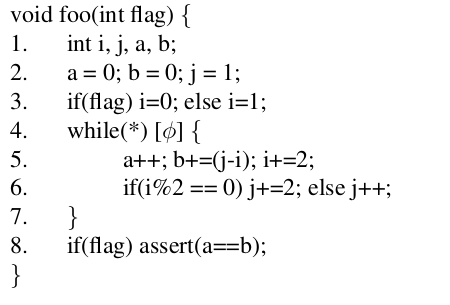
\includegraphics[scale=0.4]{exp.png}
\end{center}

1.1 Start with the weakest $\Delta_1(\phi) = true$. According to the explaination of VC: $\phi_{vc}^1 = (true\Rightarrow (\text{flag}\Rightarrow a = b))$ which is not valid ( postcondition not implied).

1.2 Find strengthening $\phi_1$, s.t. $\models true\wedge \phi_1 \Rightarrow (\text{flag}\Rightarrow a = b)$.

1.3. Candidates: $\neg \text{flag}, a = b, \text{flag}\Rightarrow a = b$.

\end{frame}

\begin{frame}\frametitle{Running Example of the Algorithm}
\begin{center}

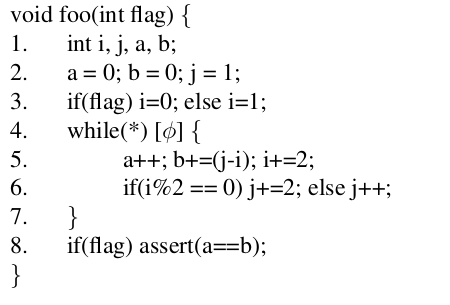
\includegraphics[scale=0.25]{exp.png}

\end{center}
1.4 Suppose $\phi_1 = (\text{flag}\Rightarrow a = b)$.

2.1 Get a new VC: $\phi_{vc}^2 = ((\text{flag}\Rightarrow a = b)\Rightarrow (\text{flag}\Rightarrow a + 1 = b + j - i))$ which is still not valid (not inductive).

2.2 Find strengthening $\phi_2$, s.t. $\models ((\text{flag}\Rightarrow a = b )\wedge \phi_2 \Rightarrow (\text{flag}\Rightarrow a + 1 = b + j - i))$.

2.3 Candidates: $\neg \text{flag}, j = i + 1, \text{flag}\Rightarrow  j = i + 1$
\end{frame}

\begin{frame}\frametitle{Running Example of the Algorithm}

\begin{center}

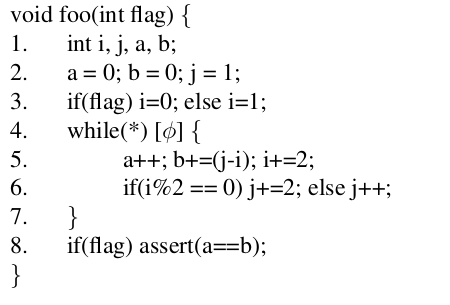
\includegraphics[scale=0.25]{exp.png}

\end{center}
1.4.1 Suppose $\phi_2 = (j = i + 1)$.

2.1 Now the candidate invariant is $(\text{flag}\Rightarrow a = b) \wedge j = i + 1$. However this is not correct one since the precondition computed does not hold on $j = i + 1$. \textbf{Backtracking}.

1.4.2 Suppose $\phi_2 = \text{flag}\Rightarrow  j = i + 1$...  

After several iterations: 

\begin{center}
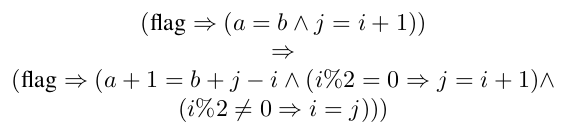
\includegraphics[scale=0.4]{resultInv.png}
\end{center}
\end{frame}


\begin{frame}\frametitle{Algorithm: InvGen}

\begin{center}
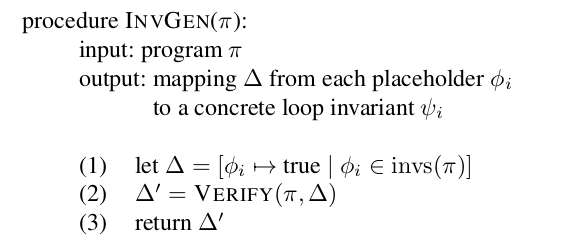
\includegraphics[scale=0.4]{main.png}
\end{center}
Here $\pi$ is the program whose syntax is:
\begin{center}

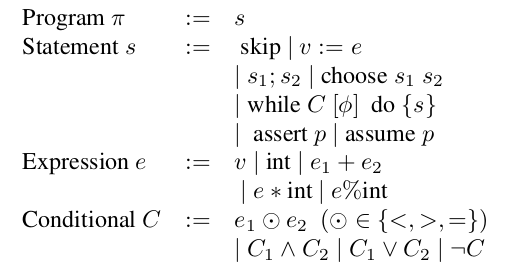
\includegraphics[scale=0.4]{prog.png}

\end{center}

\end{frame}

\begin{frame}\frametitle{Algorithm: Verify}

\begin{center}
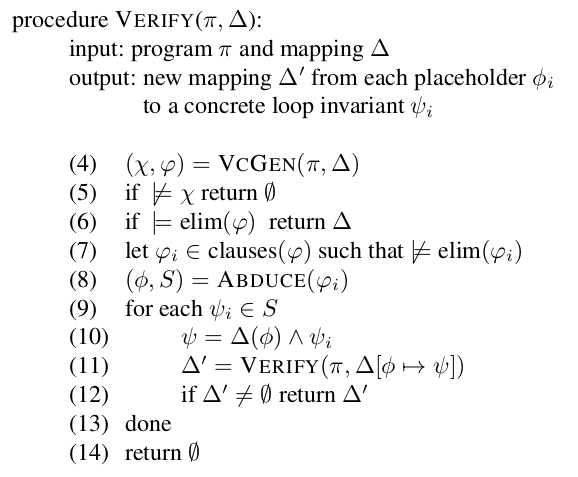
\includegraphics[scale=0.35]{verify.png}
\end{center}
elim$(\phi)$: formula that substitutes all placeholders in $\phi$ to $true$.

\end{frame}

\begin{frame}\frametitle{Algorithm: VcGen}
Input of the subprocedure \textsc{VcGen} is $\pi$ and $\Delta$, where postcondition $\chi$ can be obtained directly from $\pi$.
\[\Delta, \chi \vdash s : \chi', \phi\]
means if $\text{elim}(\phi)$ is valid, then $\{\chi'\} s \{\chi\}$ is true.
\begin{center}
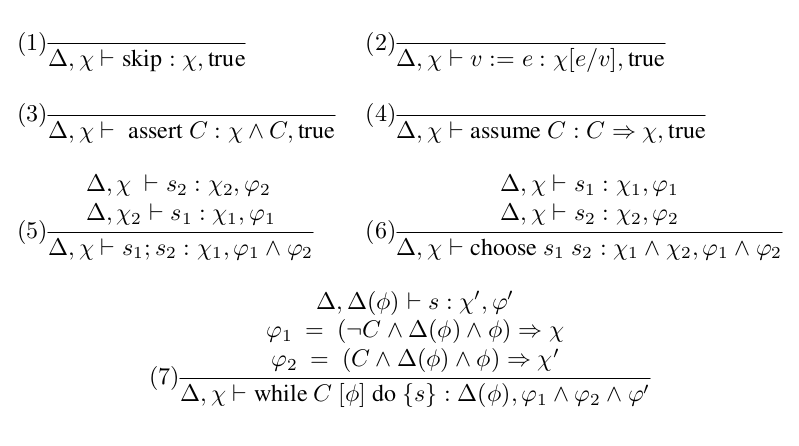
\includegraphics[scale=0.4]{inf.png}
\end{center}
\end{frame}

\begin{frame}\frametitle{Soundness of VcGen}

\begin{theorem}[Soundness]
if $\Delta, \chi \vdash s : \chi', \phi$ is derivable and $\text{elim}(\phi)$ is valid, then $\{\chi'\}s\{\chi\}$ is valid.
\end{theorem}
\begin{proof}

Prove by induction.
\begin{center}
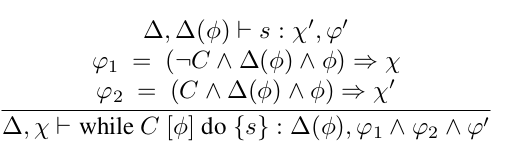
\includegraphics[scale=0.4]{loop.png}
\end{center}
\end{proof}
\end{frame}

\begin{frame}\frametitle{Algorithm: Abduce}
Recall from previous introduction of abduction: 
\begin{enumerate}
\item $(\chi\wedge \psi )\Rightarrow \gamma$

\item $\text{SAT}(\chi\wedge \psi)$
\end{enumerate}

Usually, the formula is of the form 
\[I \wedge C \Rightarrow wp(s, I)\] 
where $\chi := I \wedge C$. $\gamma := wp(s, I)$.



A direct try:  $\psi := wp(s, I)$. 

However this often causes a strengthening that is too weak and cause the divergence of the invariant.

\end{frame}

\begin{frame}\frametitle{Example: Strengthen using $wp$ introduce divergence}
\begin{multicols}{2}

\begin{center}
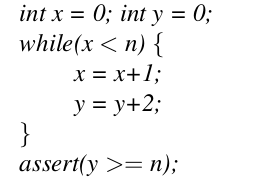
\includegraphics[scale=0.3]{diverge.png}
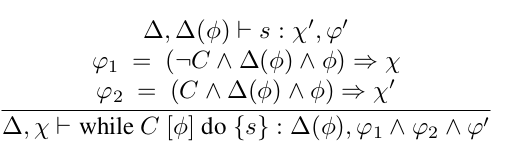
\includegraphics[scale=0.3]{loop.png}
\end{center}

\begin{enumerate}
\item Initially: $\Delta_0(\phi) = true$. VC: $x \ge n \wedge \phi \Rightarrow y\ge n$.
\item Strengthening: $\Delta_1(\phi) = (y \ge n)$. VC: $x \ge n \wedge y\ge n \wedge \phi \Rightarrow y \ge n+2$.

\item Strengthening: $\Delta_2(\phi) = (y \ge n)$. VC: $x \ge n \wedge y\ge n \wedge y \ge n+2 \wedge \phi \Rightarrow y \ge n + 4 $....

\end{enumerate}

\end{multicols}
\end{frame}

\begin{frame}\frametitle{Abduction via Quantifier Elimination}

Observation: 
\[\models (\chi\wedge \psi \Rightarrow \gamma)\]
\[\psi \models \chi\ \Rightarrow \gamma\]
\[\forall V. \chi\Rightarrow \gamma \models \chi \Rightarrow \gamma\]
where $V$ is any subset of the set of free variables $\chi\Rightarrow \gamma$.

\textbf{Goal}: try formula that is equivalent to $\forall V. \chi\Rightarrow \gamma $ and does not contradict $\chi$.

\begin{definition}[Universal Subset]
We call a set of variables $V$ a universal subset (US) of $\phi$ with respect ot $\psi$ if $(\forall V. \phi)\wedge \psi$ is satisfiable.
\end{definition}
A Universal subset $U$ is \emph{maximum} if for all other US $U'$, $|U| \ge |U'|$.
\end{frame}

\begin{frame}\frametitle{Algorithm: Abduction via QE}

\begin{center}
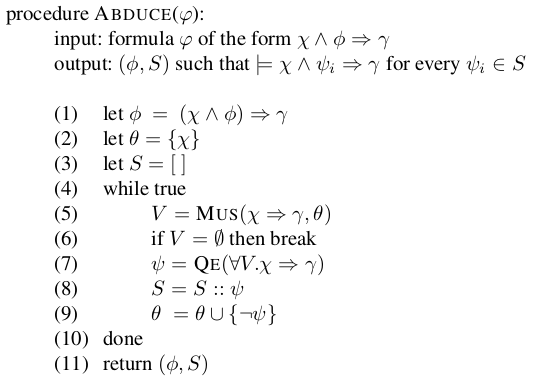
\includegraphics[scale=0.4]{abduce.png}
\end{center}
\end{frame}

\begin{frame}\frametitle{Example: Abduction via QE}
\begin{multicols}{2}

\begin{center}
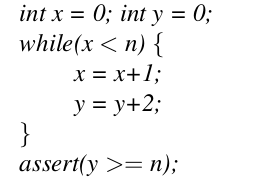
\includegraphics[scale=0.3]{diverge.png}
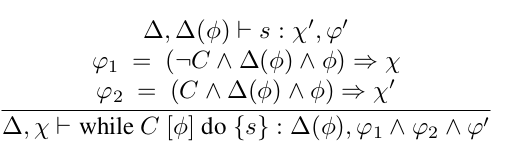
\includegraphics[scale=0.3]{loop.png}
\end{center}

\begin{enumerate}
\item Initially: $\Delta_0(\phi) = true$. VC: $x \ge n \wedge \phi \Rightarrow y\ge n$.
\item Do QE when $V = \{n\}$, $\psi := QE(\forall n. x \ge n \Rightarrow y\ge n)$. QE returns a result $y \ge x$, which is exactly the inductive loop invariant.

\end{enumerate}

\end{multicols}
\end{frame}

\begin{frame}\frametitle{Implementation Consideration}
The algorithm is implemented as a tool $\textsc{Hola}$.

Implemented in C language and use \textsc{Sail} frontend for converting from C to IR. 

Use Mistral SMT solver for satifiability solving and QE.

Features:
\begin{itemize}
\item Dual forwards and backwards analysis. 

\item Forward reasoning allow obtaining stronger inital loop invariants. 

\item Lazy abduction inference.

\end{itemize}
\end{frame}


\begin{frame}\frametitle{\textsc{Sail}}


\begin{center}
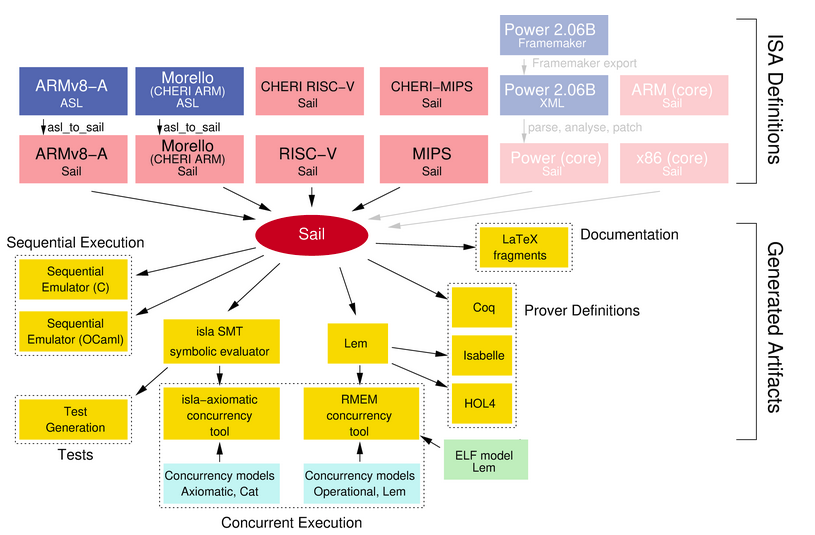
\includegraphics[scale=0.4]{sail.png}
\end{center}
\end{frame}

\begin{frame}\frametitle{Experimental Settings}
\begin{itemize}

\item Comparison with \textsc{BLAST} (CEGAR-based MC which use Craig-interpolation to generate invariants), \textsc{InvGen }(Constraint-based), \textsc{Interproc} (AI).


\item Benchmark: 46 cases.
\begin{itemize}
\item 26 are from other sources: inv. gen. papers, \textsc{InvGen} test suite, \textsc{NECLA} benchmarks.

\item 20 cases from their benchmarks.
\end{itemize}


\end{itemize}
\end{frame}

\begin{frame}\frametitle{Experimental Results}

\begin{center}
\begin{tabular}{c|c|c|c|c}
\hline 
 & \textsc{Hola} & \textsc{BLAST} & \textsc{InvGen} & \textsc{Interproc}\\
 \hline
Rate & 93.5\%&43.5\% &47.8\% &37\%\\
\hline
\end{tabular}
\end{center}

\textsc{Hola} successfully generate invariants for 13 cases where no other tools can (Divergence on other tools).

\textsc{Hola} complements the existing techniques by considering more generalized invariant and prevent divergence by QE.

There is also about 2 cases solved by others but not \textsc{Hola} (QE does not apply).

For \textsc{Hola}:
\begin{itemize}
\item Avg. 22.4 iterations.
\item Avg. 19.7 backtracking steps.

\end{itemize}
Strengthening per iteration and backtracking.

\end{frame}

\begin{frame}\frametitle{Conclusion}

\end{frame}

\begin{frame}\frametitle{Later Work \& Direction}

\begin{itemize}
\item Survey of other inv. gen. tools.
\item Survey of the toolchain \textsc{Sail}.
\end{itemize}
\end{frame}
\end{document}